\documentclass[a4paper,12pt]{report}

\def\ThesisTitle{Web Platform for Computing Principles Education}
\def\ThesisType{Master Thesis}

\def\ThesisUniversity{University of Galway}
\def\ThesisDept{College of Science and Engineering, School of Computer Science}
\def\ThesisDeptHead{Professor Michael Madden}

\def\ThesisAuthor{Jakub Duras}
\def\ThesisAdvisor{Dr Frank Glavin}

\def\ThesisPurpose{This thesis is submitted for the qualification}
\def\ThesisDegree{MSc in Software Engineering and Database Technologies}

\def\ThesisDate{\today}


% Defaults try to follow "A Guide for Graduate Research Students" from Dr. Dermot Burns, NUI Galway, 2017
% Specifically Chapter 2.5.1 Research Master's thesis layout
% https://web.archive.org/web/20210715043246/http://www.nuigalway.ie/media/graduatestudies/files/writingascientificstylethesis/writing_a_scientific_thesis.pdf

\usepackage[utf8]{inputenc}
\usepackage[british]{babel}
\usepackage{lmodern}
\usepackage[a-2u]{pdfx}

\usepackage{amsthm}                           % theorems, definitions, etc.
\usepackage{bbding}                           % various symbols (squares, asterisks, scissors, ...)
\usepackage{bm}                               % boldface symbols (\bm)
\usepackage[style=american]{csquotes}         % easier quotes
\usepackage{graphicx}                         % embedding of pictures
\usepackage{svg}                              % embedding of SVGs
\usepackage{fancyvrb}                         % improved verbatim environment
\usepackage[nottoc]{tocbibind}                % makes sure that bibliography and the lists
                                              % of figures/tables are included in the table
                                              % of contents
\usepackage{dcolumn}                          % improved alignment of table columns
\usepackage{booktabs}                         % improved horizontal lines in tables
\usepackage{paralist}                         % improved enumerate and itemize
\usepackage[en-GB]{datetime2}                 % date time utilities
\usepackage{indentfirst}                      % indent first paragraph of section
\usepackage{algpseudocode}                    % fancy pseudo code
\usepackage{fancyhdr}                         % fancy header/footer
\usepackage{setspace}                         % line spacing
\usepackage{hyphenat}                         % hyphenation control
\usepackage{titlesec}                         % custom chapter/section/subsection title style
\usepackage{hyperref}                         % links
\usepackage[acronym,toc]{glossaries}          % glossary/acronyms
\usepackage{todonotes}                        % Notes/TODOs that should get resolved
\usepackage[author={Jakub Duras}]{pdfcomment} % Comments
\usepackage{pdfpages}                         % Include other PDF
\usepackage{minted}                           % Code highlighting

\setacronymstyle{long-short}

\MakeOuterQuote{"}

% Suggestion for hyphenation can be done like com~=mu~=ni~=ty
\useshorthands{~}
\defineshorthand{~-}{\hyp{}}

% Removal of drawn-out Chapter N titles
\titleformat{\chapter}[hang]
{\normalfont\LARGE\bfseries}{\thechapter}{1em}{\LARGE}

% Sensible hyperlinks
\hypersetup{unicode}
\hypersetup{breaklinks=true}

% Assets directory
\graphicspath{ {./assets/} }

% SVG setup
\svgpath{{/assets/}}
\svgsetup{inkscapelatex=false, inkscapearea=nocrop}

% Control over floating of figure
\usepackage{float}
% Do not allow floating of figures to the next (sub)section
\usepackage[section]{placeins}
\makeatletter
\AtBeginDocument{%
  \expandafter\renewcommand\expandafter\subsection\expandafter{%
    \expandafter\@fb@secFB\subsection
  }%
}
\makeatother

% Bibliography setup to match Limerick's Cite it Right
\usepackage[style=authoryear,sorting=nyt,dashed=false,giveninits=true,uniquename=init,maxbibnames=100,maxcitenames=2,urldate=long]{biblatex}
\addbibresource{bibliography.bib}
\renewcommand{\labelnamepunct}{\addspace}
\DefineBibliographyStrings{english}{%
    andothers = {\em et\addabbrvspace al\adddot}, % Italics for et al
    available = {available},
    urlseen   = {accessed},
}
\DeclareNameAlias{sortname}{family-given} % All authors in the same order
\DeclareFieldFormat{url}{\bibstring{available}\space\url{#1}}
\DeclareFieldFormat{urldate}{[\bibstring{urlseen}\space#1]}
\NewBibliographyString{available}
\DefineBibliographyStrings{british}{available={available}}
\AtEveryBibitem{\clearfield{month}}
\AtEveryBibitem{\clearfield{day}}

% Headers and footers
\fancyhf{}
\lhead{\nouppercase{\leftmark}}
\rhead{\nouppercase{\rightmark}}
\cfoot{\thepage}
\setlength\headheight{15pt}

% Spacing between paragraphs and lines
\setlength{\parskip}{0.25em}
\onehalfspacing

% Make it very clear when the document overflows
% \overfullrule=10pt

% Custom rotate table headings
\NewDocumentCommand{\rotheading}{O{30} O{2em} m}{\makebox[#2][l]{\rotatebox{#1}{\textbf{#3}}}}


\begin{document}

\pagestyle{empty}
\begin{center}

\centerline{\mbox{
\includegraphics[width=60mm]{assets/Logo_NUIG.pdf}}}

\bigskip

{\large \ThesisUniversity}

{\ThesisDept}

\vfill

{\bfseries\Huge \ThesisTitle}

\medskip

{\Large \ThesisType}

\vspace{2cm}

{\bfseries\large \ThesisAuthor}

\medskip

{\large Advisor: \ThesisAdvisor}

\vspace{2cm}

{\large \ThesisPurpose}

\medskip

{\large \ThesisDegree}

\vspace{2cm}

\DTMlangsetup{showdayofmonth=false}
\today
\DTMlangsetup{showdayofmonth=true}

\end{center}

\cleardoublepage

\pagestyle{fancy}


\tableofcontents

\cleardoublepage

\section{Introduction}
\label{Introduction}

Understanding low-level computing principles can be beneficial for a wide variety of people - from the general public interested in computers, through practising software engineers, to Computer Science students.
Rather popular material is the open-source licensed Nand2Tetris ``taught at 400+ universities, high schools, and bootcamps" that explains how to build a computer from individual logic gates to high-level programming language \parencite{nand2tetrisweb}.
The material is accompanied by a desktop software that is hard to access or completely inaccessible from a new class of devices unsuited for desktop Java applications: Chromebooks that are seeing massive growth and now account for the majority of the US K12 market \parencite{Boreham_2019} \parencite{IDC_2021}, or mobile devices that account for 56\% of web traffic, up from only 6\% in 2011 \parencite{StatCounter_2021}.
The recently created web-based alternative, WepSIM, is showing promising results but takes a more complex look focusing on the CPU and instruction processing \parencite{garcia2019wepsim}.

Common problems with Massive Open Online Courses (MOOCs) leading to a high rate of dropouts include lack of time, problems adopting new systems, and bad past experience with technical problems on MOOC platforms \parencite{onah2014dropout}.
The use of MOOCs for software engineering education within higher education is argued to broaden student knowledge and is integrated by some universities in their courses and programmes \parencite{stikkolorum2014mooc}. However, MOOCs are also said to require significant time to both create and integrate \parencite{stikkolorum2014mooc}.

This thesis will propose a new web platform for learning computing principles involving logic gates, machine code, and assembly via a basic set of individually usable tools integrated into example content.
Can the new web platform for learning computing principles improve student task success rate compared to commonly used desktop software like that of Nand2Tetris?

\section{Scope and Significance of Research}

This thesis will explore material for learning computing principles and accompanied software, the state of the MOOCs and their shortcomings, and current best practices on creating and maintaining open-source software.

The mentioned exploration will feed into the design, development, and evaluation of a new web application.
There are several deliverables expected at the end of the research:

\begin{enumerate}
    \item[A] Simple web platform accessible from all major devices without any setup, including Chromebooks, tablets, and smartphones. It will feature the ability to sign in, retain the progress, and share the state of individual tools.
    \item[B] Reimagined web version of Hardware Simulator, Hack Computer, and Hack Assembler from Nand2Tetris running solely on the client-side web. These will be usable standalone and embedded.
    \item[C] Content management for the web platform via Markdown files hosted at Github with the first half of the CC-licensed Nand2Tetris content as a starting point.
    \item[D] Primary data on selected objective User Experience (UX) metrics useful for judging usability in and out of classrooms - completion rate, time on task, and the number of problems/frustrations. 
\end{enumerate}

These deliverables should be useful to all three groups of people mentioned in the \nameref{Introduction}. Specifically, these deliverables will be usable as:

\begin{itemize}
    \item Easily accessible alternative software for the Nand2Tetris course available at Coursera \footnote{Build a Modern Computer from First Principles: From Nand to Tetris (Project-Centered Course), URL: \url{https://www.coursera.org/learn/build-a-computer}}. The software will be shared with the community and proposed as an alternative to users struggling to run the original software, e.g., Chromebook, tablet, smartphone, Windows S users, and users lacking permissions or experience to install Java.
    \item Individual tools that can be integrated into traditional education. Since the tools will be kept as simple as possible, they should be usable with relatively low time investment.
    \item A standalone platform for self-education of computing principles with the starting content and ability to extend it as people see fit, thanks to its open nature.
    \item An example showing attainable accessibility and efficiency improvements from moving desktop education tools to the web.
\end{itemize}

\begin{figure}[h!]
    \centering
    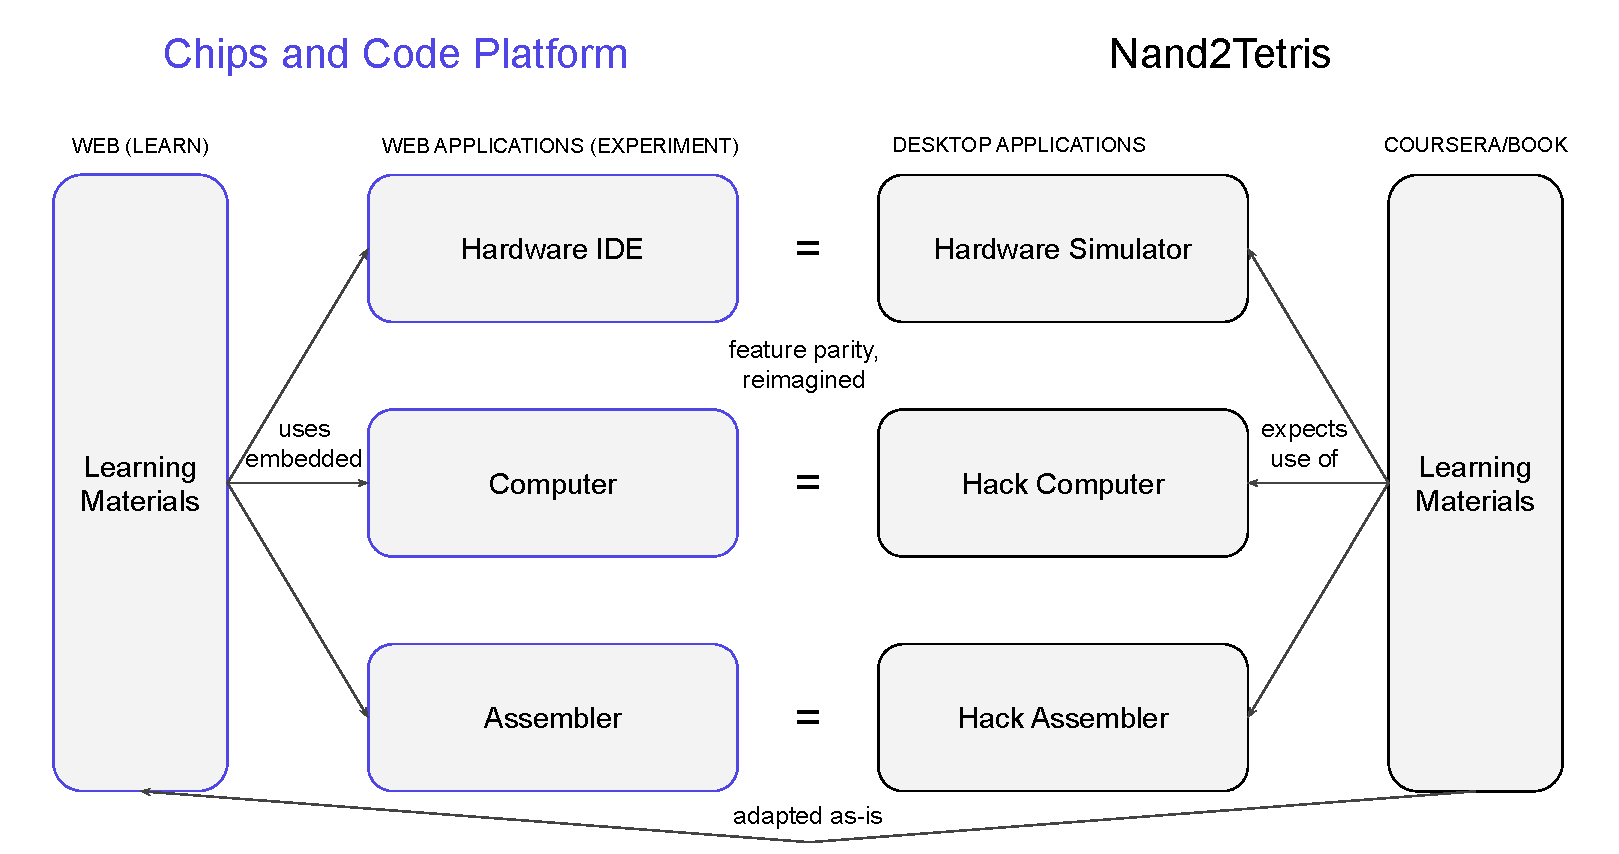
\includegraphics[width=\textwidth]{Comparison_Architecture}
    \caption{Overview of deliverables and their relation to Nand2Tetris.}
\end{figure}

\section{Methodology}

The main paradigm used for this thesis will be Design Science Research (DSR), as currently outlined by \parenciteyear{brocke2020designscience}.
It will use existing theories, frameworks, and models to produce and evaluate a new artefact - instantiation, as categorised by \parenciteyear{hevner2004designscience}.

The evaluation of the artifact will consist of two parts:

\begin{itemize}
    \item \textbf{Automated Tests}
    It is assumed it will be possible to achieve feature parity with the selected three tools.
    To evaluate this and confirm the feasibility of porting to the client-side web, the author will prepare two classes of automated tests: end-to-end and unit tests.
    End-to-end tests will focus on the ability to perform equivalent actions (feature-parity) and unit tests, among else, to confirm various inputs, including the Nand2Tetris assignments from all six weeks, can be used and produce correct output (correctness).
    \item \textbf{Primary Quantitative Research}
    The central hypothesis is that the increased efficiency from using the web instead of the desktop will increase the student task success rate.
    This will be evaluated by conducting a comparative study.
    The participants will be tasked to perform a simple exercise of implementing chips like AND and NAND or XOR and XNOR in Nand2Tetris and the newly developed platform.
    The order of implemented gates and used programs will be randomised, and participants will be from different backgrounds corresponding to three target demographics mentioned in the \nameref{Introduction} - Computer Science students, practitioners with/without formal education, and people interested, but not directly involved, in Computer Science.
    The tasks will be performed in their home environment corresponding to currently widespread distance learning or self-learning and will include the setup of the software.
    Collected data will include objectively measurable UX task metrics: completion rate, time on task, and the number of problems/frustrations.
\end{itemize}

\begin{figure}[h!]
    \centering
    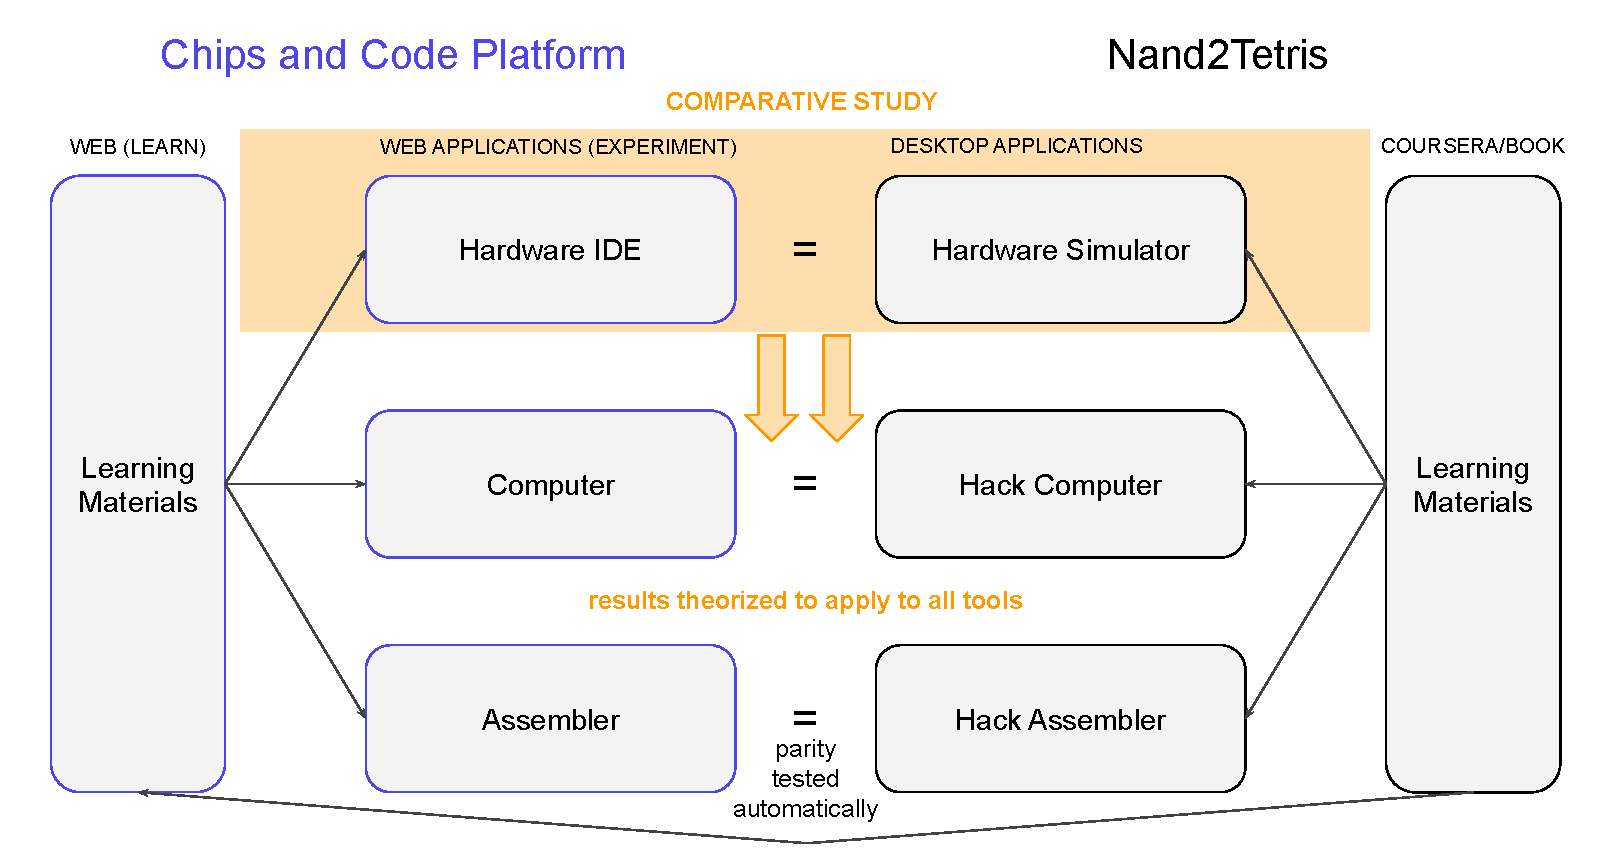
\includegraphics[width=\textwidth]{Comparison_Evaluation}
    \caption{Overview of evaluated parts.}
\end{figure}

Collected knowledge will be interpreted and described as part of the discussion.
It is expected unstructured qualitative data could be generated in the process, e.g., the experience of participants using and integrating the system and their feedback.
If that happens to be the case and the data will be significant enough, they will be documented as part of the discussion. However, this thesis will not delve into qualitative data.

\section{Success Criteria}

The thesis completion will be assessed based on the following criteria:

\begin{itemize}
    \item The literature review covers all research identified in the beginning.
    It could be measured by looking at each identified research - was it read and were appropriate actions taken as a result - incorporated into the thesis or transformed into a task on design, development, or evaluation.
    \item Planned functionality that was broken down into tasks during the literature review is implemented, at least 80\% of the major functionality is covered by automated tests, and tests pass.
    \item The conducted study has collected enough data to be statistically significant with a group size of at least 12 \parencite{macefield2009specify}. Collected data have been processed and incorporated into the thesis.
\end{itemize}

\section{Thesis Project Plan}

Figure~\ref{fig:tasklist} shows identified deliverables and Figure~\ref{fig:ganttchart} their planning. Deliverables are managed using GitHub, which can also be used for planning.

\begin{figure}[h!]
    \centering
    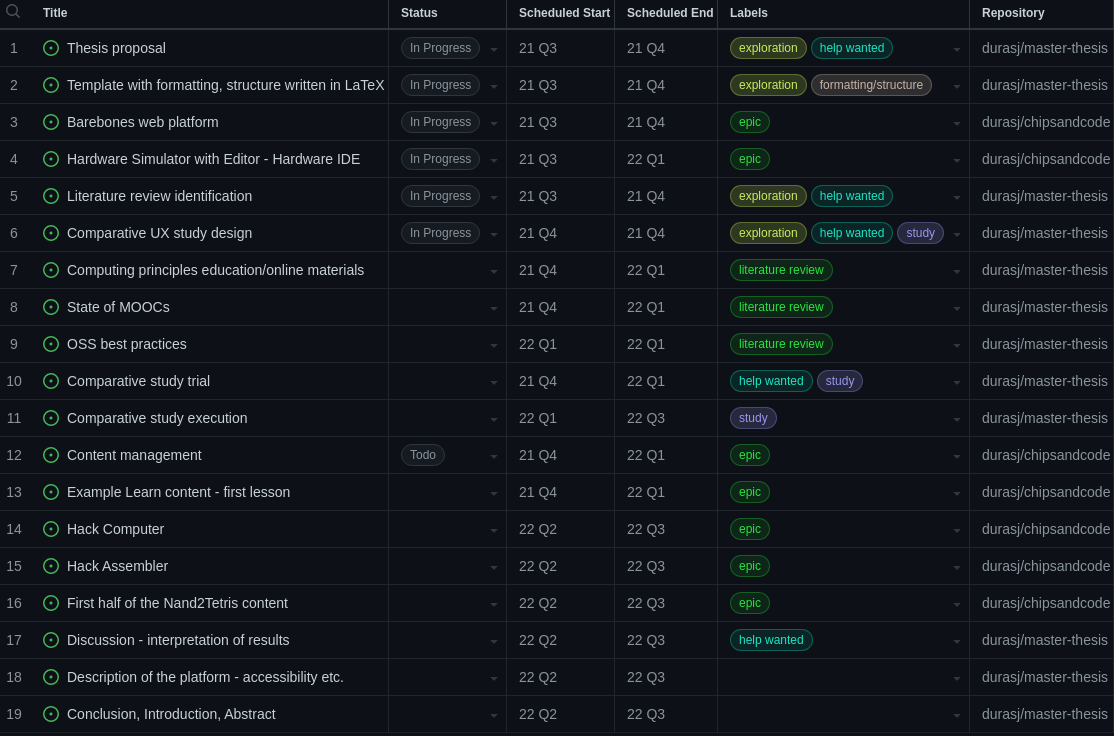
\includegraphics[width=\dimexpr(\textheight-10em), angle=90]{Task_List}
    \caption{Deliverables for Thesis Project Plan as screenshot from GitHub.}
    \label{fig:tasklist}
\end{figure}

\begin{figure}[h]
    \centering
    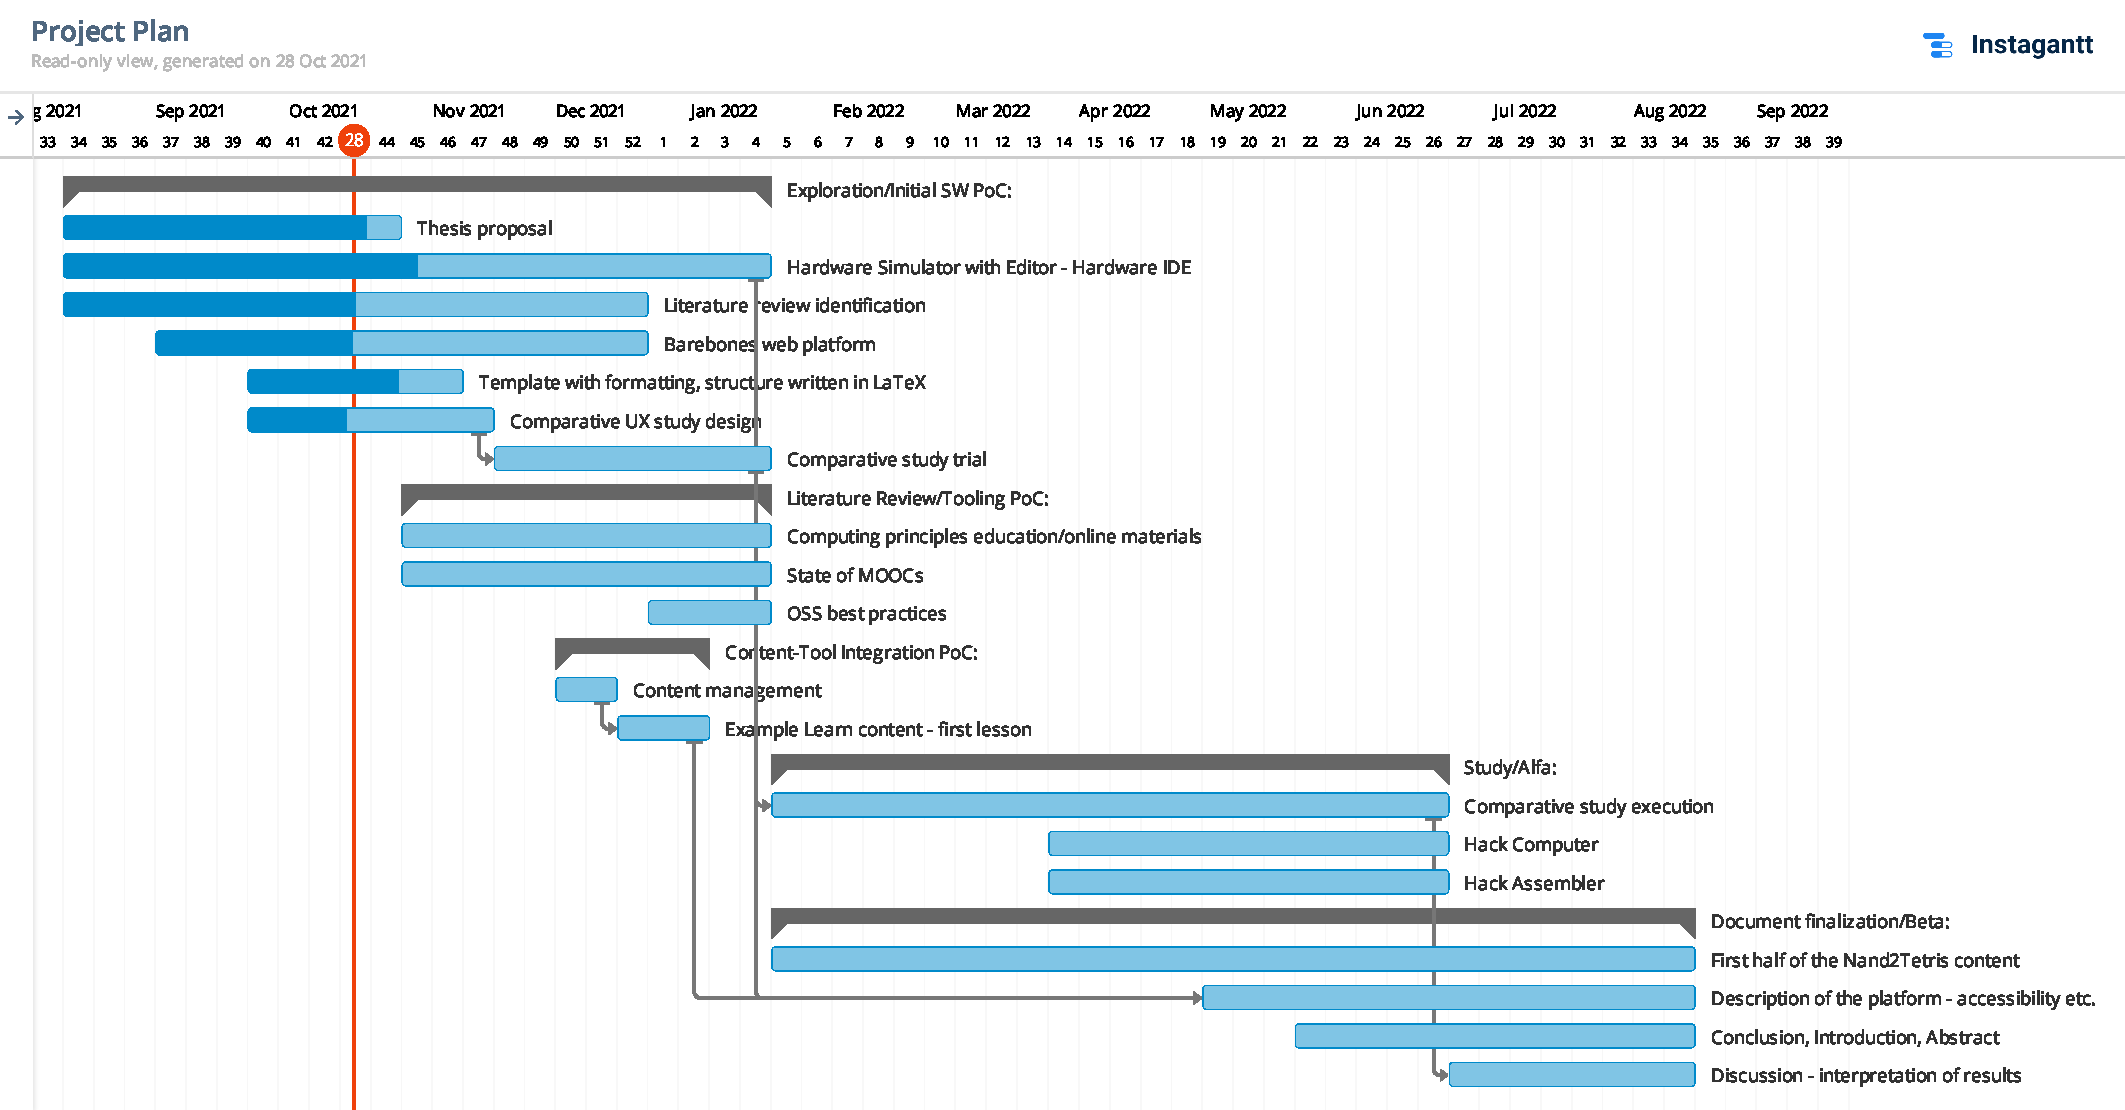
\includegraphics[width=\dimexpr(\textheight-1em), angle=90]{Gantt_Chart}
    \caption{Gantt Chart for Thesis Project Planning.}
    \label{fig:ganttchart}
\end{figure}

\cleardoublepage

\printbibliography[heading=subbibintoc]

\end{document}
